\documentclass[conference]{IEEEtran}
\IEEEoverridecommandlockouts
\usepackage{setspace}
\usepackage{gensymb}
\singlespacing
\usepackage[cmex10]{amsmath}
\usepackage{amsthm}
\usepackage{mathrsfs}
\usepackage{txfonts}
\usepackage{stfloats}
\usepackage{bm}
\usepackage{cite}
\usepackage{cases}
\usepackage{subfig}
\usepackage{longtable}
\usepackage{multirow}
\usepackage{enumitem}
\usepackage{mathtools}
\usepackage{tikz}
\usepackage{circuitikz}
\usepackage{verbatim}
\usepackage[breaklinks=true]{hyperref}
\usepackage{tkz-euclide} % loads  TikZ and tkz-base
\usepackage{listings}
\usepackage{color}    
\usepackage{array}    
\usepackage{longtable}
\usepackage{calc}     
\usepackage{multirow} 
\usepackage{hhline}   
\usepackage{ifthen}   
\usepackage{lscape}     
\usepackage{chngcntr}
\usepackage{algorithm}
\usepackage[indLines=false]{algpseudocodex}
\DeclareMathOperator*{\Res}{Res}
\renewcommand\thesection{\arabic{section}}
\renewcommand\thesubsection{\thesection.\arabic{subsection}}
\renewcommand\thesubsubsection{\thesubsection.\arabic{subsubsection}}

\renewcommand\thesectiondis{\arabic{section}}
\renewcommand\thesubsectiondis{\thesectiondis.\arabic{subsection}}
\renewcommand\thesubsubsectiondis{\thesubsectiondis.\arabic{subsubsection}}
\renewcommand\thetable{\arabic{table}}
% correct bad hyphenation here
\hyphenation{op-tical net-works semi-conduc-tor}
\def\inputGnumericTable{}                                 %%

\renewcommand\algorithmicensure{\textbf{Input:}}
\newcommand{\algorithmautorefname}{Algorithm}
\renewcommand{\sectionautorefname}{Section}

\lstset{
%language=C,
frame=single, 
breaklines=true,
columns=fullflexible,
literate=
{-}{$\rightarrow{}$}{1},
}
%\lstset{
%language=tex,
%frame=single, 
%breaklines=true
%}

\DeclareMathOperator*{\argmax}{arg\,max}
\DeclareMathOperator*{\argmin}{arg\,min}
\begin{document}
\newtheorem{theorem}{Theorem}[section]
\newtheorem{problem}{Problem}
\newtheorem{proposition}{Proposition}[section]
\newtheorem{lemma}{Lemma}[section]
\newtheorem{corollary}[theorem]{Corollary}
\newtheorem{example}{Example}[section]
\newtheorem{definition}[problem]{Definition}
\newcommand{\BEQA}{\begin{eqnarray}}
\newcommand{\EEQA}{\end{eqnarray}}
\newcommand{\define}{\stackrel{\triangle}{=}}
\providecommand{\mbf}{\mathbf}
\providecommand{\pr}[1]{\ensuremath{\Pr\left(#1\right)}}
\providecommand{\qfunc}[1]{\ensuremath{Q\left(#1\right)}}
\providecommand{\sbrak}[1]{\ensuremath{{}\left[#1\right]}}
\providecommand{\lsbrak}[1]{\ensuremath{{}\left[#1\right.}}
\providecommand{\rsbrak}[1]{\ensuremath{{}\left.#1\right]}}
\providecommand{\brak}[1]{\ensuremath{\left(#1\right)}}
\providecommand{\lbrak}[1]{\ensuremath{\left(#1\right.}}
\providecommand{\rbrak}[1]{\ensuremath{\left.#1\right)}}
\providecommand{\cbrak}[1]{\ensuremath{\left\{#1\right\}}}
\providecommand{\lcbrak}[1]{\ensuremath{\left\{#1\right.}}
\providecommand{\rcbrak}[1]{\ensuremath{\left.#1\right\}}}
\theoremstyle{remark}
\newtheorem{rem}{Remark}
\newcommand{\sgn}{\mathop{\mathrm{sgn}}}
\providecommand{\abs}[1]{\left\vert#1\right\vert}
\providecommand{\res}[1]{\Res\displaylimits_{#1}} 
\providecommand{\norm}[1]{\left\lVert#1\right\rVert}
\providecommand{\mtx}[1]{\mathbf{#1}}
\providecommand{\mean}[1]{E\left[ #1 \right]}   
\providecommand{\fourier}{\overset{\mathcal{F}}{ \rightleftharpoons}}
\providecommand{\system}[1]{\overset{\mathcal{#1}}{ \longleftrightarrow}}
\newcommand{\solution}{\noindent \textbf{Solution: }}
\newcommand{\cosec}{\,\text{cosec}\,}
\providecommand{\dec}[2]{\ensuremath{\overset{#1}{\underset{#2}{\gtrless}}}}
\newcommand{\myvec}[1]{\ensuremath{\begin{pmatrix}#1\end{pmatrix}}}
\newcommand{\mydet}[1]{\ensuremath{\begin{vmatrix}#1\end{vmatrix}}}
\renewcommand{\vec}[1]{\boldsymbol{\mathbf{#1}}}
\def\putbox#1#2#3{\makebox[0in][l]{\makebox[#1][l]{}\raisebox{\baselineskip}[0in][0in]{\raisebox{#2}[0in][0in]{#3}}}}
     \def\rightbox#1{\makebox[0in][r]{#1}}
     \def\centbox#1{\makebox[0in]{#1}}
     \def\topbox#1{\raisebox{-\baselineskip}[0in][0in]{#1}}
     \def\midbox#1{\raisebox{-0.5\baselineskip}[0in][0in]{#1}}

\title{Indoor Wireless Beacon Tracking Using ESP32}
\author{
    \IEEEauthorblockN{Gautam Singh, Sachin Omprakash Dubey, G.V.V. Sharma} \\
    \IEEEauthorblockA{Indian Institute of Technology Hyderabad, India} 
    %\IEEEauthorblockA{Indian Institute of Technology Hyderabad, India} \\
}
\maketitle

\begin{abstract}
    Through this paper, we demonstrate the use of machine learning in
    beacon tracking using an unmanned ground vehicle (UGV) and a WiFi-enabled
    microcontroller such as the ESP32.
    This is done by using received signal strength indicator (RSSI) values from a single target beacon as inputs to the microcontroller. These values are then used for making decisions on UGV positioning using learning algorithms. 
\end{abstract}

\section{Introduction}
\label{sec:intro}
Positioning, localization and navigation (PLAN) technology has become an
essential capability for consumer electronics and autonomous vehicles alike.
This fast growing market has seen the entry of big technology industry that was traditionally focused on internet software \cite{}.  
Use cases of PLAN include safety, medical applications and
assistance for the elderly and the specially abled \cite{}. Reliable PLAN technology can
reduce road accidents, congestion, energy and time consumption. However, many
existing PLAN technologies cater to industrial use cases and are expensive,
complex and require hardware that might be scarcely available to consumers \cite{}. 

To overcome the above challenges, we propose a simple, effective and robust
algorithm for indoor beacon tracking using a single WiFi or BLE beacon and a
low-cost easily available microcontroller such as the ESP32 that is suitable for
consumer electronics such as robot vacuum cleaners. The main contributions of
this paper are as follows.

\begin{enumerate}
    \item A simple yet robust algorithm for indoor beacon tracking using only
    RSSI measurements from a single target beacon.
    \item A practical implementation of the algorithm on an ESP32
    microcontroller mounted on a UGV chassis using open-source frameworks such
    as PlatformIO.
\end{enumerate}

The remainder of this paper is organized as follows. In
\autoref{sec:related-work}, we present a brief survey of related work in the
field of indoor beacon tracking. In \autoref{sec:proposed-system}, we formulate
the optimization problem corresponding to this task and describe our approach.
In \autoref{sec:implementation}, we present the implementation details of the
algorithm on the ESP32 microcontroller. In \autoref{sec:results}, we present the
experimental results and performance evaluation of our proposed approach.
Finally, in \autoref{sec:conclusion}, we conclude the paper and discuss possible
extensions of our work.

\section{Related Work}
\label{sec:related-work}

A comprehensive survey of PLAN technology presented in
\cite{el-sheimyIndoorNavigationState2021} categorizes PLAN technologies based on
the primary sensors used in navigation and illustrates the trade-offs between
accuracy, cost and complexity. Some of these technologies are briefly described
below.

A fuzzy
controller system  consisting of three ultrasonic sensors and one camera to
detect obstacles in the robot's vicinity is presented in \cite{narayananFuzzyGuidedAutonomous2022}. The navigation logic is implemented on
BLE tag modules using the angle of arrival (AOA) method and is suitable for
unmanned nursing in hospitals, especially during pandemic outbreaks. \cite{familiIDROPRobustLocalization2023} proposes iDROP, a 3D localization
scheme for drones in indoor GPS-denied environments that is robust against noise
and multipath fading and provides location estimation with high accuracy. A UGV implemented on the
robot operating system (ROS) that uses light detection and ranging (LiDAR) for
accurate navigation even in dynamic conditions and is suitable for various
indoor robotic use cases such as in warehouses or construction sites is available in \cite{htROSPoweredAutonomous2024}. \cite{yukhimetsLocalNavigationSystem2024} proposes a scalable
navigation system using multiple ESP32 microcontrollers acting as BLE beacons. Here, a 
neural network models the position of the robot based on the signal strength
received from the various beacons and the Levenberg-Marquardt method is used to
accurately estimate the position of the robot. 
%A strategy for landing a UAV is discussed in \cite{stefasUAVLandingUnknown2019}This uses a
%radio beacon that exploits a special structure occurring when approaching the
%target beacon from above to reduce the flight time required for landing near the
%beacon.

Methods based on artificial intelligence (AI) have gained popularity in recent
literature. \cite{liuSimpleOnlineUnmanned2021} proposes an easy to
implement method for multi-object tracking (MOT) using an encoder-decoder
mechanism. The proposed method achieves comparable performance with
state-of-the-art frameworks on the challenging MOT dataset. In
\cite{masmitjaReinforcementLearningPath2022}, deep reinforcement
learning (RL) is leveraged to train an agent for tracking dynamically moving objects using
unmanned surface vehicles (USV) in marine environments. The trained RL agent
performs comparably to the analytically derived trajectory in the steady state.
The authors of \cite{kashyapAutonomousNavigationROS22025} explore multiple RL
algorithms using LiDAR inputs on TurtleBot3, showing that the twin delayed deep
deterministic policy gradient (TD3) is the most efficient and robust across
varied environments.

Many of the above methods are either too complex or too expensive to be
implemented on cheap hardware such as an ESP32 microcontroller. Furthermore, a
lot of supporting infrastructure needs to be set up to enable autonomous
navigation. Our work aims to address these challenges by providing a lightweight
and cost-effective solution for indoor beacon tracking using a single wireless
beacon and easily available wireless-capable microcontrollers such as the ESP32.

\section{Proposed Navigation System}
\label{sec:proposed-system}

In this section, we formulate the beacon tracking problem as an optimization
problem. We propose two solutions to this problem and compare their effectiveness.

%Then, we describe our algorithm for solving this optimization problem
%using gradient ascent and compare it to a similar algorithm proposed in
%\cite{dubeyNavigationCommunicationUGV2022}.

\subsection{Problem Statement}
\label{subsec:problem-statement}

To estimate (radial) distance to beacon, we use its signal strength which is
usually given by the Received Signal Strength Indicator (RSSI). The RSSI (in
dBm) at radial distance of \(r\) metres is defined as
\begin{align}
    R\brak{r} = R\brak{1} - 10\log_{10}\brak{r},
    \label{eq:rssi}
\end{align}
where \(R\brak{1}\) is the RSSI at a distance of 1 metre from the beacon. Using
this definition, the beacon tracking problem can be formulated as the following
optimization problem.
\begin{equation}
    \max_{r} R\brak{r} \text{ s.t. } r > 0.
    \label{eq:rssopt}
\end{equation}
The derivative and second derivative of \(R\brak{r}\) is
\begin{align}
    R^\prime\brak{r} &= -\frac{10}{\ln{10}}\frac{1}{r}, \label{eq:rssid} \\
    R^{\prime\prime}\brak{r} &= \frac{10}{\ln{10}}\frac{1}{r^2} > 0. \label{eq:rssidd}
\end{align}
Notice that for \(r > 0\), \(R^\prime\brak{r} < 0\), thus \(R\brak{r}\) is a
decreasing function of \(r\). This implies that the maximum RSSI is at \(r =
0\), as expected. Since \(R\brak{r}\) is a convex function of \(r\), we can use
gradient ascent \cite{boydConvexOptimization2004a} to recursively find the point
where the RSSI is maximum, which would correspond to the location of the beacon.
Using \eqref{eq:rssid}, the gradient ascent update equation for the radial
distance \(r\) is given by
\begin{equation}
    r_{n+1} = r_n + \alpha R^\prime\brak{r_n} = r_n - \frac{10\alpha}{r_n\ln{10}}
    \label{eq:gradient-ascent-upd}
\end{equation}
where \(r_i\) is the radial distance at the \(i\)-th step and \(\alpha\) is the
step size and \(r_0\) is the initial radial distance of the UGV. Since \(r_n >
0\), we can see that \(r_{n+1} < r_n\) for all \(n\). In other words, the radial
distance to the beacon is decreasing with each step. This means that the UGV
will converge towards the beacon. However, due to the explosion of the gradient
in \eqref{eq:rssid} at \(r = 0\), the update steps become larger as \(r_n\)
decreases, which could lead to overshooting the beacon. We now compare two
algorithms that overcome this limitation by using a recursive approach that
keeps the step size constant.

\subsection{Beacon Tracking Algorithm}
\label{subsec:beacon-tracking-algorithm}

It builds upon the algorithm proposed in
\cite{dubeyNavigationCommunicationUGV2022}.
The proposed beacon tracking algorithm consists of two stages at each step. The
first stage is the \emph{probing stage}, where the UGV measures the RSSI at
various points in its vicinity. The second stage is the \emph{decision stage},
where the UGV decides its direction of movement based on the RSSI measurements.
We now discuss an existing algorithm that follows this approach of recursively
probing and subsequent decision making and compare it with our proposed
algorithm.

\subsubsection{Existing Algorithm}
\label{subsubsec:existing-algorithm}

The algorithm proposed in \cite{dubeyNavigationCommunicationUGV2022} is
described in \autoref{alg:beacon-dubey}. The probing phase consists of taking
RSSI measurements in place but at various orientations. The decision phase
consists of moving in the direction where the signal is the strongest. A major
drawback of this approach is that there may not be appreciable difference in the
measured RSSI values at the various orientations in the same place, especially
if the beacon is far away. This could lead to the UGV making arbitrary moves
instead of converging towards the beacon.

\begin{algorithm}[H]
    \caption{Beacon Tracking Algorithm of \cite{dubeyNavigationCommunicationUGV2022}.}
    \label{alg:beacon-dubey}
    \begin{algorithmic}[1]
        \Ensure{RSSI threshold \(T\), number of steps \(N\)}
        \While{\textsc{GetRSSI()} \(< T\)}
            \State \(r_F \gets \textsc{GetRSSI()}\).
            \State Turn left by 90 degrees in place.
            \State \(r_L \gets \textsc{GetRSSI()}\).
            \State Turn right (from initial orientation) by 90 degrees in place.
            \State \(r_R \gets \textsc{GetRSSI()}\).
            \If{\(r_F \ge r_L\) and \(r_F \ge r_R\)}
                \State Turn to the initial direction in place.
            \ElsIf{\(r_L \ge r_F\) and \(r_L \ge r_R\)}
                \State Turn to the left direction in place.
            \Else{\(r_R \ge r_F\) and \(r_R \ge r_L\)}
                \State Turn to the right direction in place.
            \EndIf
            \State Move forward in the chosen direction by one step.
        \EndWhile
    \end{algorithmic}
\end{algorithm}

\subsubsection{Proposed Algorithm}
\label{subsubsec:proposed-algorithm}

To overcome the issue of arbitrary movement when placed at a large distance from
the beacon, the UGV must travel a significant distance in the probing stage to
obtain differences in the measured RSSI values so that there is enough
information to make a decision that is better than movement in a randomly chosen
direction. Thus, in the probing stage of our proposed algorithm, the UGV
measures the RSSI at \(N\) points in a straight line in its current orientation.
In the decision stage, the UGV then moves to the position where the maximum RSSI
was measured. If this is at the beginning or end of the probing trajectory, the
UGV moves backward or forward respectively. Otherwise, it turns perpendicular to
its probing trajectory at that point (either left or right). Our proposed
algorithm is described in \autoref{alg:beacon}. The main shortcoming of this
particular algorithm is the amount of movement required in the probing stage for
making one simple move in the decision stage.

\begin{algorithm}[H]
    \caption{Proposed Beacon Tracking Algorithm}
    \label{alg:beacon}
    \begin{algorithmic}[1]
        \Ensure{RSSI threshold \(T\), number of points \(N\)}
        \While{\textsc{GetRSSI()} \(< T\)}
            \State \(r_0 \gets \textsc{GetRSSI()}\).
            \For{i = 1 to \(N - 1\)}
                \State Move forward by one step.
                \State \(r_i \gets \textsc{GetRSSI()}\).
            \EndFor
            \State \(j \gets \argmax_{i} r_i\).
            \State Move to the position at step \(i\).
            \If{\(i = N - 1\)}
                \State Move one step forward.
            \ElsIf{\(i = 0\)}
                \State Move one step backward.
            \Else
                \State Turn left.
            \EndIf
        \EndWhile
    \end{algorithmic}
\end{algorithm}

\section{Implementation}
\label{sec:implementation}

Source codes for both of the beacon tracking algorithms discussed above are
implemented in C++. They are available on
\href{https://github.com/goats-9/ee2802/main/ugv-beacon/codes}{GitHub}.

\subsection{Assets}
\begin{enumerate}
    \item UGV chassis with DC motors
    \item ESP32 microcontroller with Type-B USB cable
    \item L293D Motor Driver IC
    \item Breadboard and Jumper Wires
    \item Android phone
    \item (Optional) USB 2.0/3.0 Hub
\end{enumerate}

\subsection{Procedure}
\begin{enumerate}
    \item Make the connections as per the wiring diagram in
    \autoref{fig:beacon}.
    \item Connect the ESP32 board to your Android Phone.
    \item Generate the firmware by entering the following commands.
        \begin{lstlisting}
$ cd codes
$ pio run
        \end{lstlisting}
    \item Go to ArduinoDroid and select
        \begin{lstlisting}
Actions - Upload - Upload Precompiled
        \end{lstlisting}
    and choose the firmware file at
        \begin{lstlisting}
codes/.pio/build/firmware.hex
        \end{lstlisting}
    \item Now put the phone at a reasonable distance from the UGV with no
    obstacles in the way and then turn on the hotspot. The UGV should travel
    towards the phone and stop near it.
\end{enumerate}

\begin{figure}[t]
    \centering
    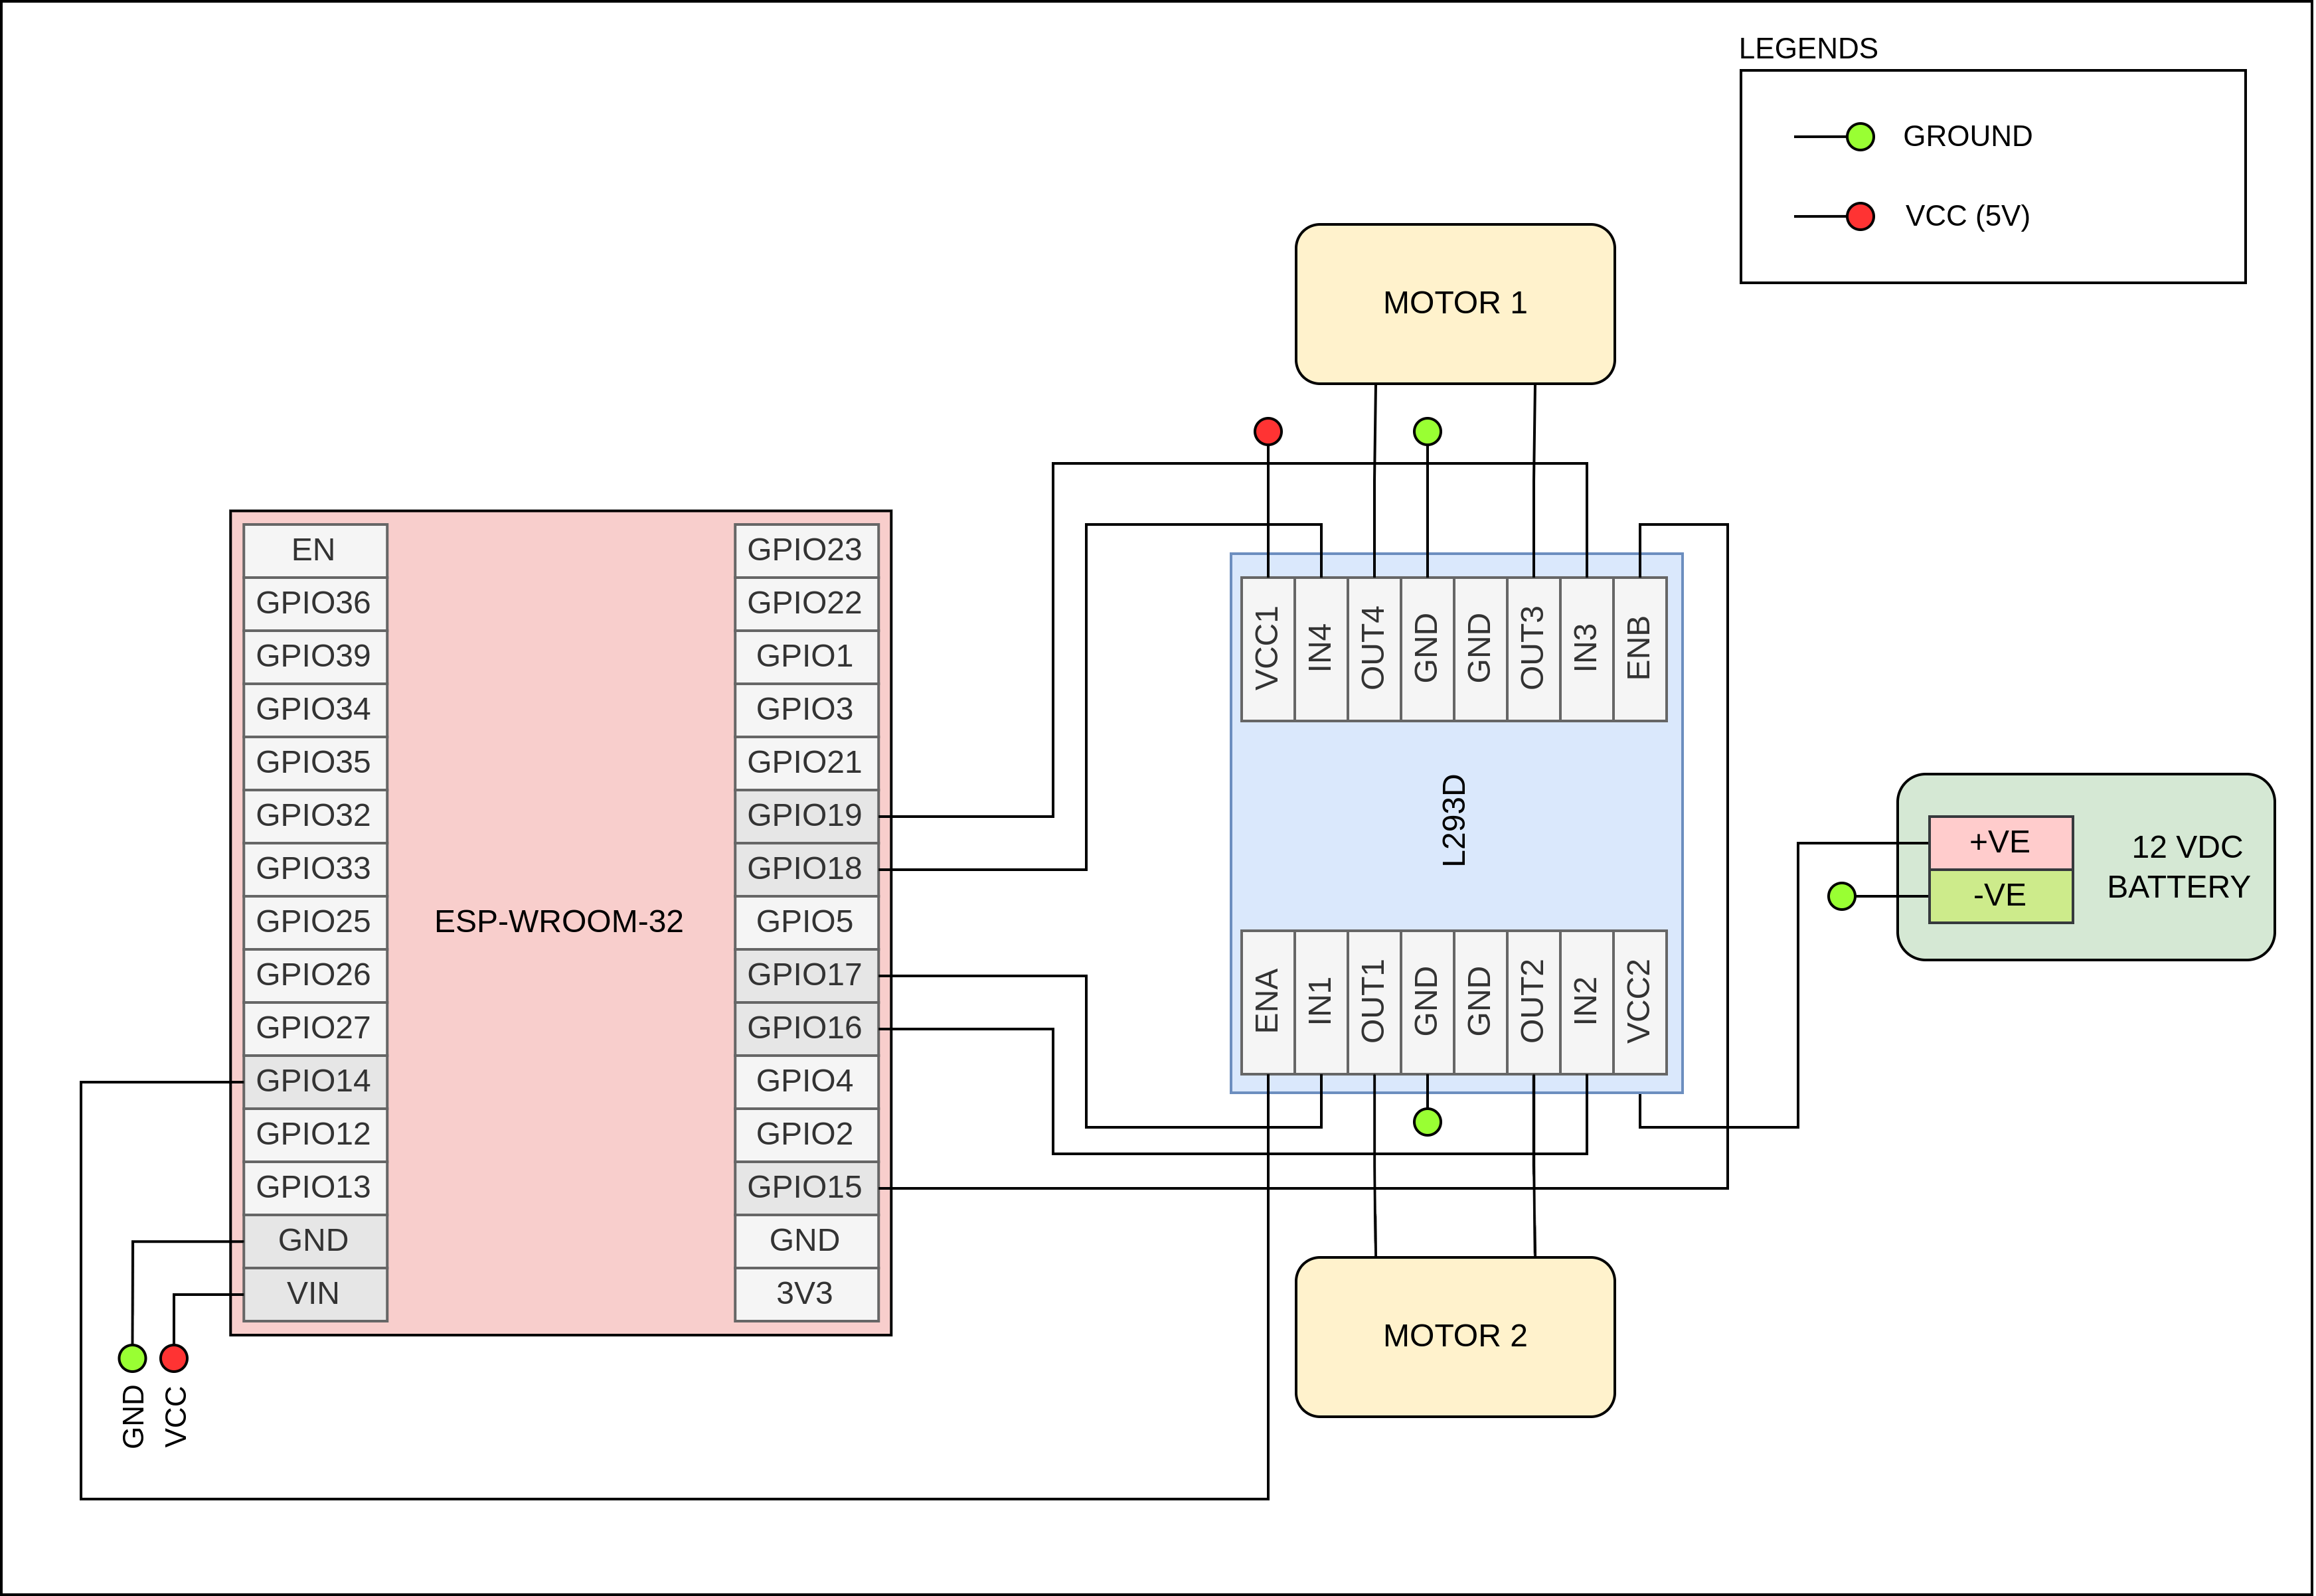
\includegraphics[width=\columnwidth]{figs/beacon.png}
    \caption{Wiring Diagram for Beacon Tracking.}
    \label{fig:beacon}
\end{figure}

\section{Results}
\label{sec:results}
The UGV eventually converges close to the beacon (here, the hotspot). However,
if there are a lot of nearby obstacles, the UGV may not converge close to the
location of the beacon. It may either get physically blocked by the beacon or
the signal interference may be too high.

\section{Conclusion and Future Work}
\label{sec:conclusion}

In this paper, we presented a cost-effective and robust beacon tracking
algorithm that uses RSSI measurements to approach the beacon at each step. Our
work uses easily available hardware and software tools to implement the
algorithm on an ESP32 microcontroller mounted on a UGV chassis. A simple
extension to our proposed algorithm could be to reduce the time and total number
of steps taken by adjusting the value of \(N\) as the UGV converges to the
beacon. This could be done using various heuristics such as the total number of
probes or current RSSI measurements. A further extension of this work could be
to use additional sensors such as a gyroscope or an accelerometer to improve the
accuracy of the UGV's position and prevent deviations from the intended path of
the UGV.

\bibliographystyle{IEEEtran}
\bibliography{references}

\end{document}
